% HMC Math dept HW template example
% v0.04 by Eric J. Malm, 10 Mar 2005
\documentclass[12pt,letterpaper,boxed,cm]{hmcpset}

% set 1-inch margins in the document
\usepackage[margin=1in]{geometry}
\usepackage{mathtools}
\usepackage{mathrsfs}
% include this if you want to import graphics files with /includegraphics
\usepackage{graphicx}
\usepackage{cases}
\usepackage{hyperref}
\usepackage{siunitx}
\usepackage{tikz}
\usetikzlibrary{arrows}

% info for header block in upper right hand corner
\name{Name: ~~~~~~~~~~~~~~~~~~~~~~~~~}
\class{Physics 51}
\assignment{Homework \#6}
\duedate{September 19, 2016}

\newcommand{\ev}[2]{\Big|_{#1}^{#2}}
\newcommand{\evv}[2]{\Big|_{#1}^{#2}}
\newcommand{\set}[1]{\left\{#1\right\}}
\newcommand{\s}[1]{\sqrt{#1}}
\newcommand{\f}[2]{\frac{#1}{#2}}
\newcommand{\p}[2]{\frac{\partial #1}{\partial #2}}
\providecommand{\t}[1]{\text{#1}}
\providecommand{\span}[1]{\text{span}\left(#1\right)}
\providecommand{\set}[1]{\left\{#1\right\}}
\providecommand{\l}[0]{\left}
\providecommand{\r}[0]{\right}
\newcommand{\m}[1]{\begin{matrix}#1\end{matrix}}
\newcommand{\bm}[1]{\begin{bmatrix}#1\end{bmatrix}}
\renewcommand{\bf}[1]{\mathbf{#1}}
\newcommand{\pn}[1]{\left( #1 \right)}
\newcommand{\abs}[1]{\left| #1 \right|}
\newcommand{\bk}[1]{\left[ #1 \right]}
\newcommand{\cis}[1]{\pn{\cos\pn{#1} + i\sin\pn{#1}}}
\newcommand{\cisi}[1]{\pn{\cos\pn{#1} - i\sin\pn{#1}}}
\renewcommand{\Im}[1]{\text{Im}\pn{#1}}
\renewcommand{\Re}[1]{\text{Re}\pn{#1}}
\renewcommand{\k}[0]{\f{1}{4\pi\epsilon_0}}

\makeatletter
\renewcommand*\env@matrix[1][*\c@MaxMatrixCols c]{%
  \hskip -\arraycolsep
  \let\@ifnextchar\new@ifnextchar
  \array{#1}}
\makeatother
\begin{document}
\problemlist{28-P8, 28-P11, 28-P13, SUP4*}

\begin{problem}[28-P8]	
Figure 28-42 shows, edge-on, an "infinite" sheet of positive charge density $\sigma$.
\begin{enumerate}
	\item[(a)] How much work is done by the electric field of the sheet as a small positive test charge $q_0$ is moved from an initial position on the sheet to a final position located a perpendicular distance $z$ from the sheet?
	\item[(b)] Use the result from (a) to show that the electric potential of an infinite sheet of charge can be written
	\[
		V = V_0 - \pn{\sigma/2\epsilon_0}z,
	\]
	where $V_0$ is the potential at the surface of the sheet.
\end{enumerate}
\begin{center}
	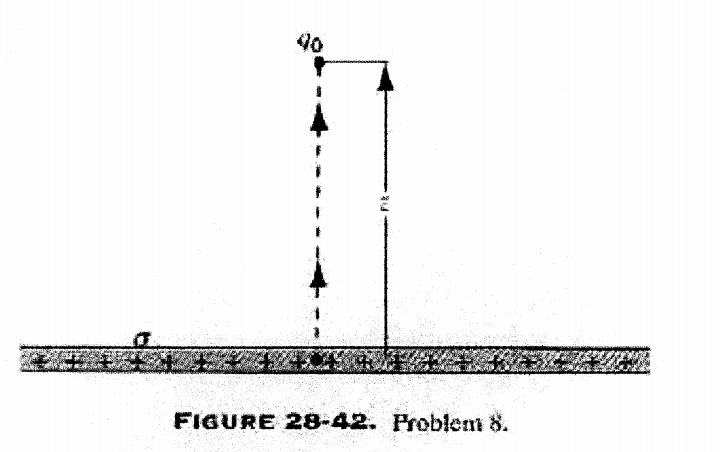
\includegraphics[scale=0.7]{01.png}
\end{center}
\end{problem}
\begin{solution}
\end{solution}
\newpage


\begin{problem}[28-P11]
For the charge configuration of Fig. 28-44, show that $V(r)$ for points on the vertical axis, assuming $r \gg d$, is given by
\begin{equation*}
	V = \k \f{q}{r} \pn{1 + \f{2d}{r}}.
\end{equation*}
(Hint: The charge configuration can be viewed as the sum of an isolated charge and a dipole.) Set $V = 0$ at infinity.
\begin{center}
	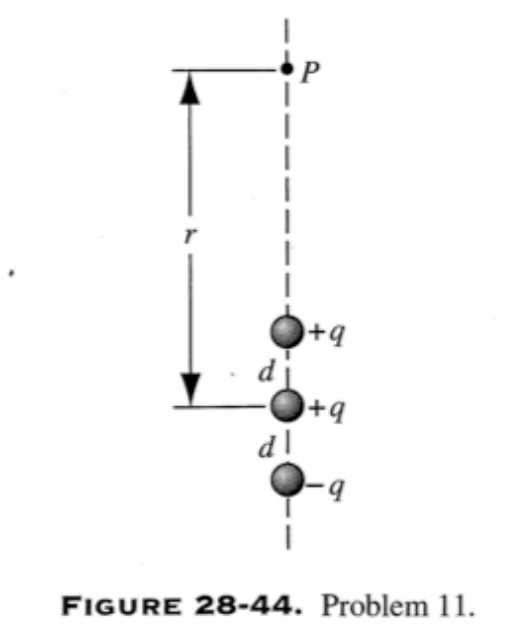
\includegraphics[scale=0.7]{02.png}	
\end{center}
\end{problem}
\begin{solution}	
\end{solution}
\newpage


\begin{problem}[28-P13]
On a thin rod of length $L$ lying along the $x$ axis with one end at the origin ($x = 0$), as in Fig. 28-46, there is a distributed a charge per unit length given by $\lambda = kr$, where $k$ is a constant and $r$ is the distance from the origin.
\begin{enumerate}
	\item[(a)] Taking the electrostatic potential at infinity to be zero, find $V$ at the point $P$ on the $y$ axis.
	\item[(b)] Determine the vertical component, $E_y$, of the electric field at $P$ from the result of part (a) and also by direct calculation.
	\item[(c)] Why cannot $E_x$, the horizontal component of the electric field at $P$, be found using the result of part (a)?
	\item[(d)] At what distance from the rod along the $y$ axis is the potential equal to one-half the value at the left end of the rod?
\end{enumerate}	
\begin{center}
	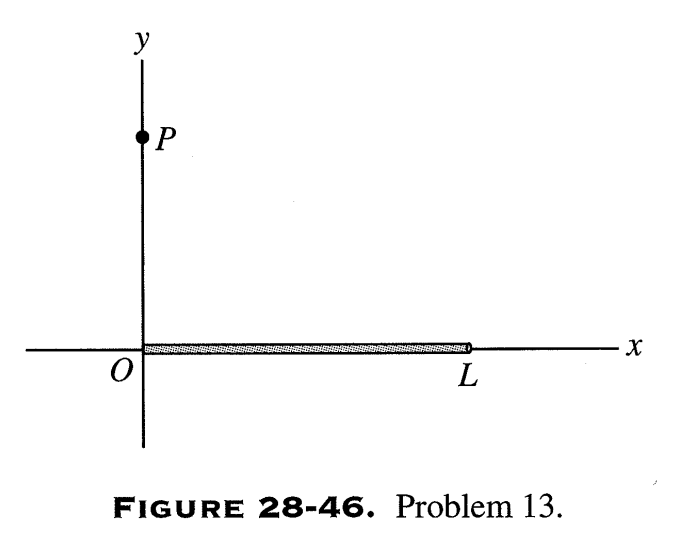
\includegraphics[scale=0.7]{03.png}
\end{center}
\end{problem}
\begin{solution}
\end{solution}
\newpage


\begin{problem}[SUP4*]
	\begin{enumerate}
		\item[(a)] Calculate the energy density of the electric field at a distance $r$ from an electron (presumed to be a particle) at rest.
		\item[(b)] Assume now that the electron is not a point but a sphere of radius $R$ over whose surface the electron charge is uniformly distributed. Determine the energy associated with the external electric field in vacuum of the electron as a function of $R$.
		\item[(c)] If you now associate this energy with the mass of the electron, you can, using $E_0 = mc^2$, calculate a value for $R$. Evaluate this radius numerically; it is often called the \textit{classical radius} of the electron.
	\end{enumerate}
\end{problem}
\begin{solution}
\end{solution}

\end{document}
